\section{Motor Controller}
The motor controller consists of two parts.
The first is the Arduino Mega 2560, located in a black box underneath the laptop, on top of the batteries.
The second are two rotary encoders \cite{roten}, located on the two front wheels.
These are wired to the arduino via 2 gray ribbon cables.

\subsection{Arduino Mega 2560}
This was already a part of the solution before the 2019 Q1 \& Q2 group started work on the project.
Using the pre-existing connections made by previous groups where old rotary encoders were attached, the new rotary encoders have been connected.

\subsection{Rotary Encoders}
These rotary encoders were chosen based on the following criteria:

\begin{itemize}
\item Encoders must have a resolution of at least 1024 PPR \ref{trm::PPR}
\item Encoders must run of a 3.3 or 5V current
\item Encoders must be attachable to the wheels, either through pre-fabricated attachments or 3d-printable sockets
\item Encoders must be priced within the budget provided by the product owner
\item Encoders must be able to record both directions
\end{itemize}

The Bourns encoders chosen satisfy all the given criteria.
While the documentation states that there are 256 cycles per revolution, each cycle produces 4 pulses.
This adds up to 1024 Pulses Per Revolution.


\subsubsection{Flexible Coupling}
The rotary encoders have been socketed on the axles using a 3-d printed mount, using the coupling shown in fig \ref{fig::FCR}.

\begin{figure}[H]
\centering
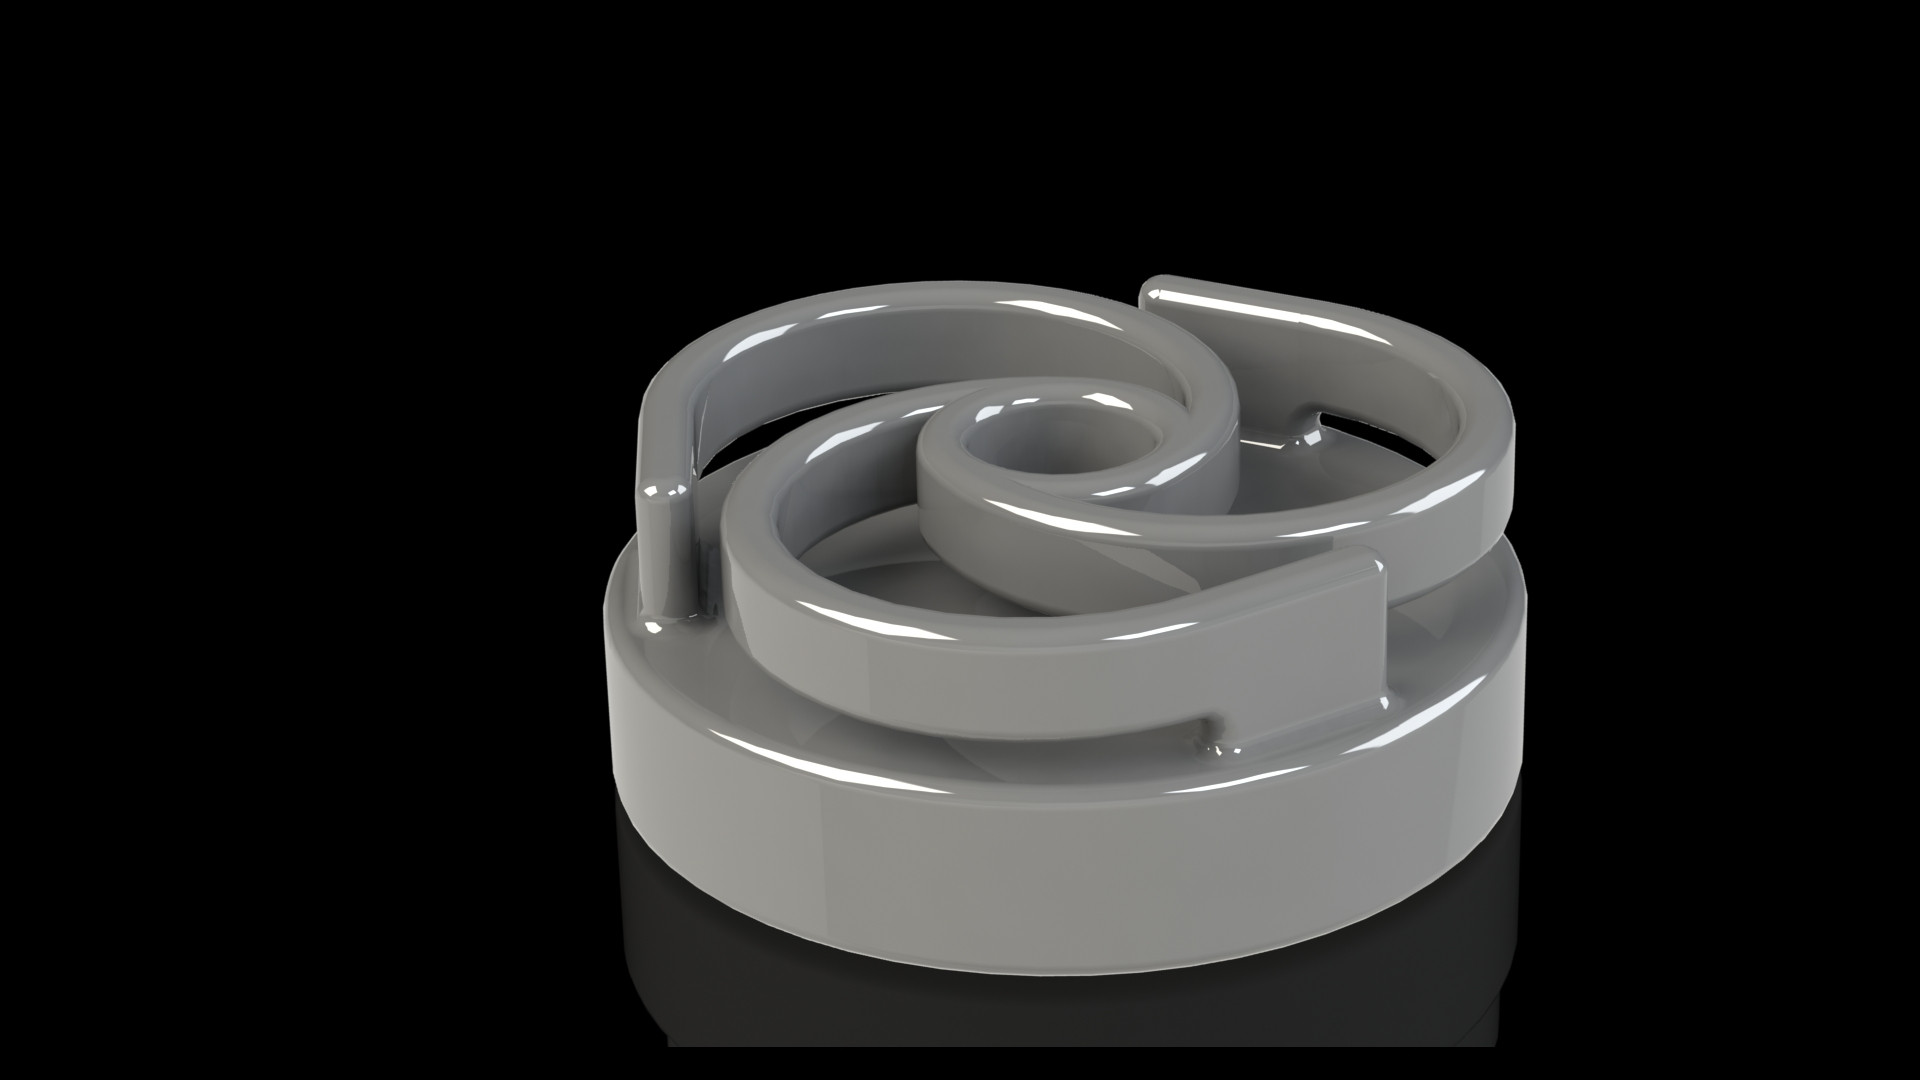
\includegraphics[width=12cm]{FlexibleCouplingRender1.JPG}
\caption{The flexible coupling for the rotary encoder}
\label{fig::FCR}
\end{figure}

The full assembly is as shown in fig \ref{fig::REA}

\begin{figure}[H]
\centering
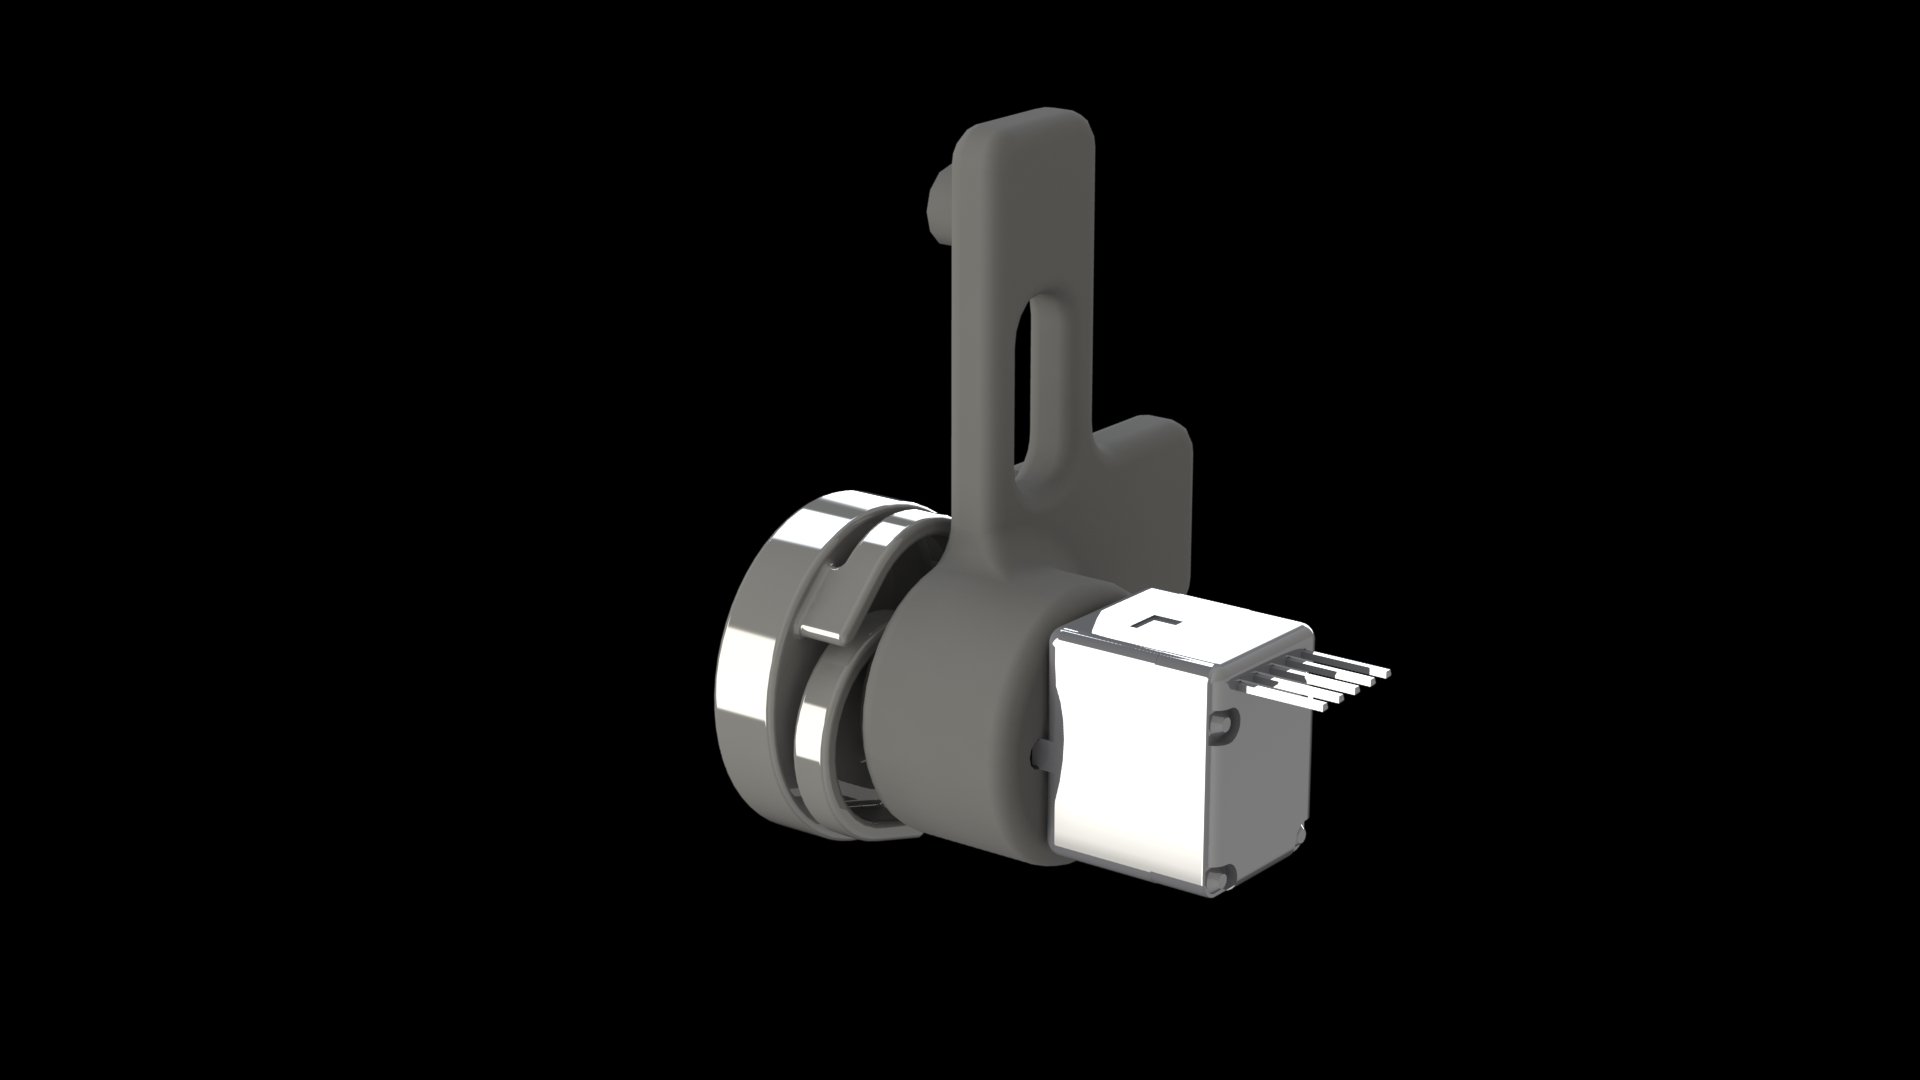
\includegraphics[width=12cm]{RotaryEncoderAssembly1.JPG}
\caption{Full assembly of the mount for the rotary encoders}
\label{fig::REA}
\end{figure}

The flexible coupling provides 5 degrees of freedom.
The coupling allows the axis to move slightly in lateral directions as relative to the axle, as well as slightly towards and away from the axle.
This has been tested in Solidworks, and a 10N force is enough to move the axle 0.5mm.

\subsubsection{Wiring}
The wiring for the encoders on the Arduino side was already in place, due to the old encoders that were since removed.
Figure \ref{fig::WD} shows the wiring.

\begin{figure}[H]
\centering
\includegraphics[width=12cm]{something.image}
\caption{The wiring of the rotary encoders}
\label{fig::WD}
\end{figure}



